\section{Обзор существующих методов аугментации изображений для задачи распознавания рукописного текста}
\label{sec:Chapter2} \index{Chapter2}

\begin{figure}
    \centering
    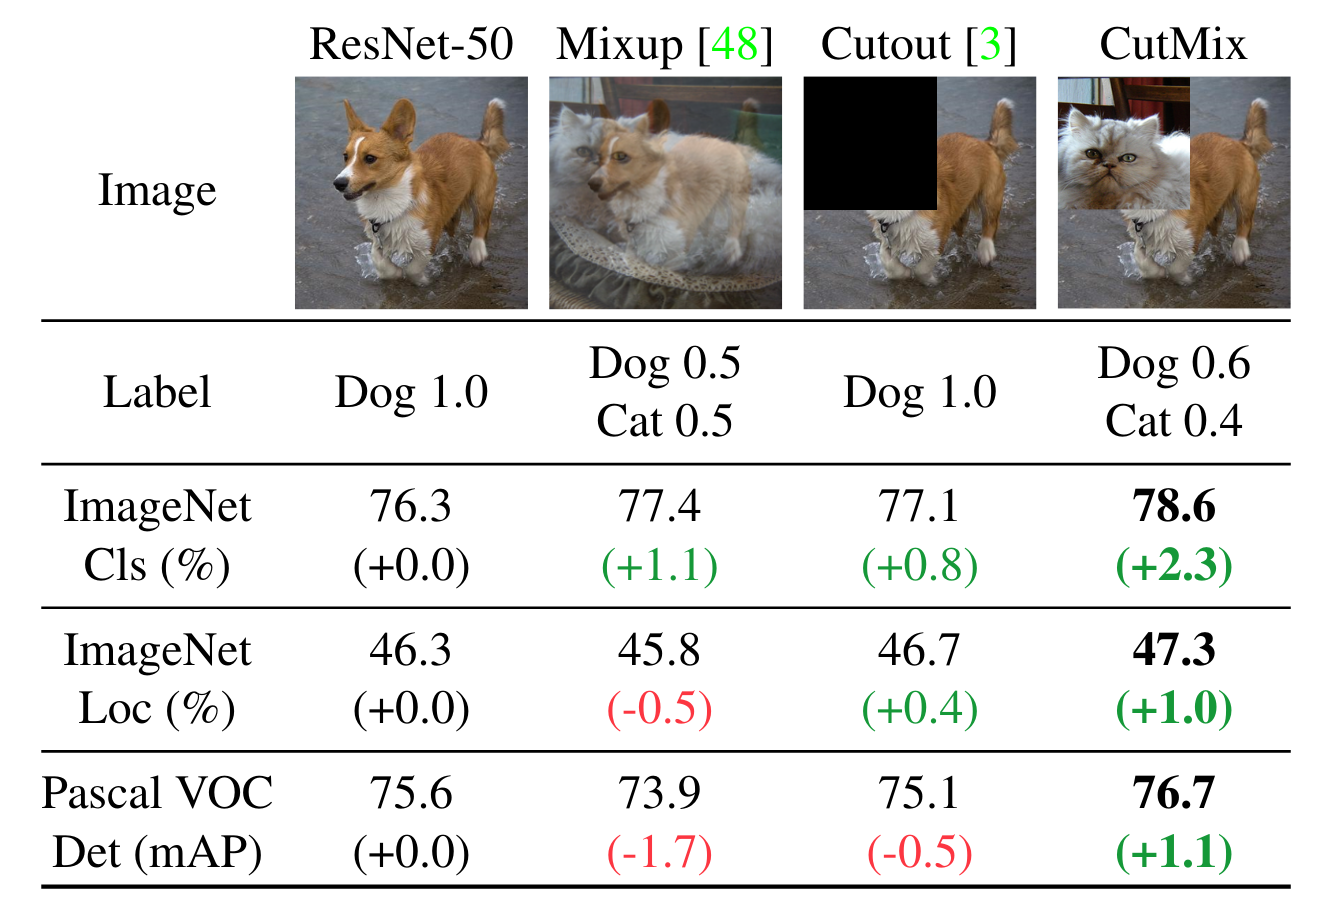
\includegraphics[scale=0.25]{./images/cutmix.png}
    \caption{\protect\hypertarget{image7}{Результаты различных техник аугментаций на ImageNet. \\ Взято из \protect\hyperlink{cite.Yun19}{[26]}}.}
\end{figure}

Помимо распространенных техник аугментации, которые используются в широком спектре задач компьютерного зрения, таких как:
\begin{enumerate}
\item отражение по горизонтали/вертикали,
\item повороты и угловые трансформации,
\item изменение масштаба,
\item добавление шума,
\item обрезка,
\item цветовые преобразования,
\item искажения различных форм,
\end{enumerate}
существуют также методы аугментации, которые специфически применяются для решения определенных задач. Далее будут описаны некоторые из таких методов аугментации. В каждом из рассмотренных видов аугментации новые объекты создаются путем комбинирования двух или более объектов из набора данных.

\subsection{CutMix}
Пусть $x \in \mathbb{R}^{W \times H \times C}$ и $y$ обозначают изображение и его целевую переменную соответственно. Целью метода CutMix является создание нового образца $(\tilde{x}, \tilde{y})$ путем комбинирования двух образцов $(x_A, y_A)$ и $(x_B, y_B)$. \hyperlink{image7}{[Рис 7.]} Созданный образец $(\tilde{x}, \tilde{y})$ используется для обучения модели с использованием ее исходной функции потерь. Операция комбинирования определяется следующим образом:
\begin{equation}
\begin{split}
\tilde{x} = M \odot x_A + (1 - M) \odot x_B \\
\tilde{y} = \lambda y_A + (1 - \lambda) y_B,
\end{split}
\end{equation}
где $M \in {0, 1}^{W \times H}$ обозначает бинарную маску, $1$ - бинарная маска, заполненная единицами, и $\odot$ - покомпонентное умножение. $\lambda$ выбирается из бета-распределения $Beta(\alpha, \alpha)$. В отличие от mixup \hyperlink{cite.Hon17}{[25]}, CutMix \hyperlink{cite.Yun19}{[26]} заменяет область изображения патчем из другого обучающего изображения и создает более локально естественное изображение.

Для выборки бинарной маски $M$ мы сначала выбираем координаты ограничивающего прямоугольника $B = (r_x, r_y, r_w, r_h)$. Область $B$ в $x_A$ удаляется и заполняется частью, обрезанной из $B$ на $x_B$. Выбираются прямоугольные маски M, соотношение сторон которых пропорционально оригинальному изображению. Координаты прямоугольников выбираются равномерно в соответствии со следующим правилом:
\begin{equation}
\begin{split}
r_x \sim Unif (0, W), r_w = W \sqrt{1 - \lambda} \\
r_y \sim Unif (0, H), r_h = H \sqrt{1 - \lambda}
\end{split}
\end{equation}
соотношение площадей картинок есть 
\begin{equation}
\frac{r_w r_h}{WH} = 1 - \lambda
\end{equation}
На каждой итерации обучения CutMix-образец ($\tilde{x}, \tilde{y}$) генерируется путем комбинирования случайно выбранных двух образцов в батче.

\begin{figure}
    \centering
    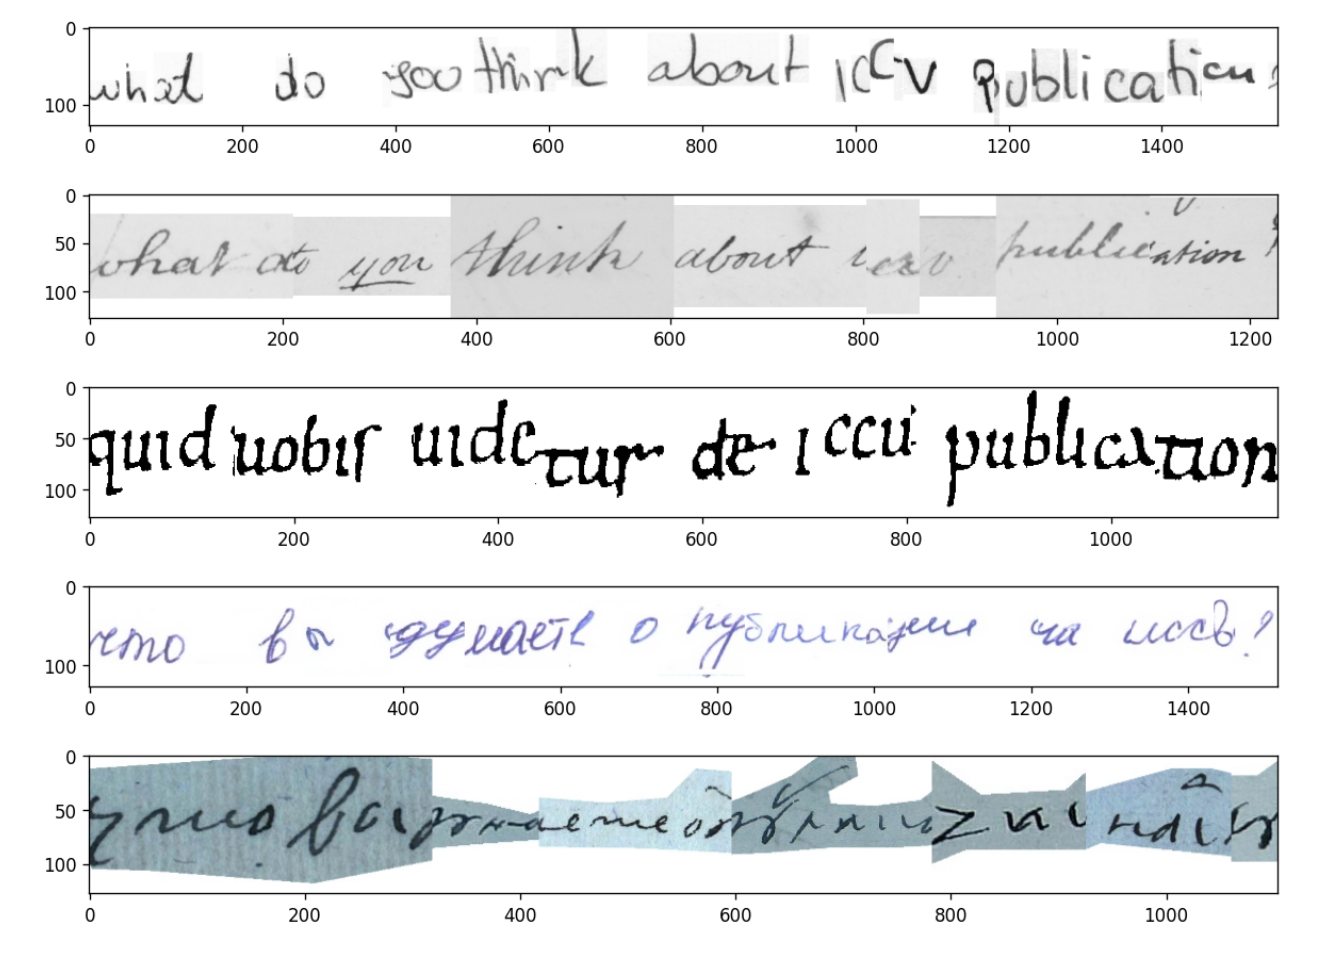
\includegraphics[scale=0.25]{./images/stackmix.png}
    \caption{\protect\hypertarget{image8}{Примеры изображений, созданных с помощью StackMix. \\ Взято из \protect\hyperlink{cite.Sho21}{[27]}.}}
\end{figure}

\subsubsection{StackMix}
В \hyperlink{cite.Sho21}{[27]} этот подход был адаптирован для задачи распознавания рукописного текста. В StackMix различные фрагменты рукописного текста склеиваются в некотором порядке. \hyperlink{image8}{[Рис 8.]}

Чтобы применить предложенный подход к задаче распознавания рукописного текста, требуется дополнительная разметка данных, которая точно отмечает границы символов. Для достижения этой цели используется подход с автоматической сегментацией обучающих изображений на символы с использованием постобработки контролируемой предварительно обученной нейронной сети (с декодером Connectionist Temporal Classification). 

\begin{figure}
    \centering
    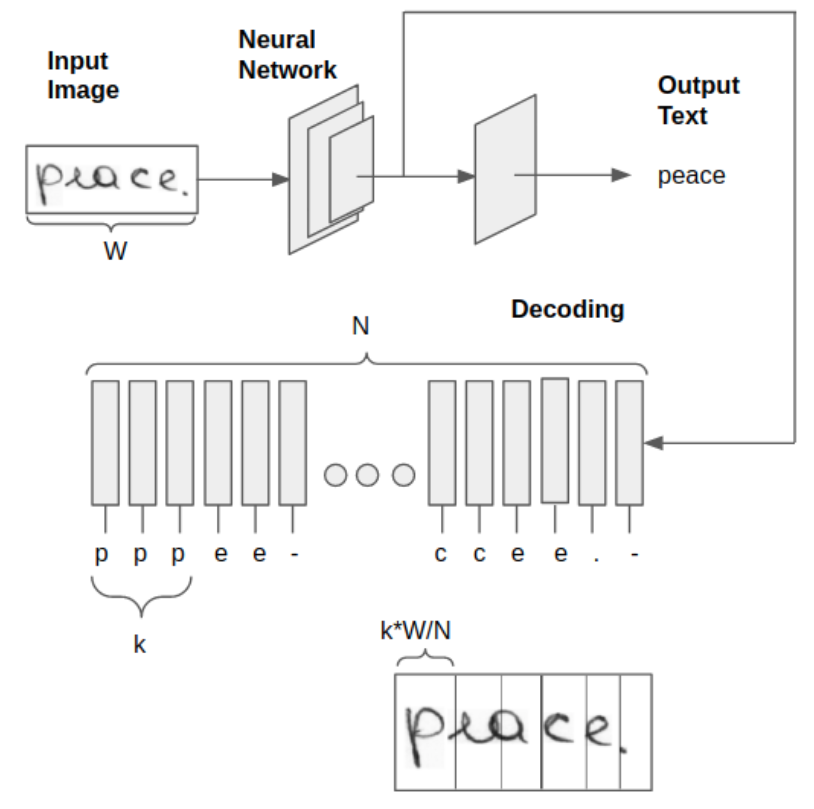
\includegraphics[scale=0.25]{./images/stackmix_algo.png}
    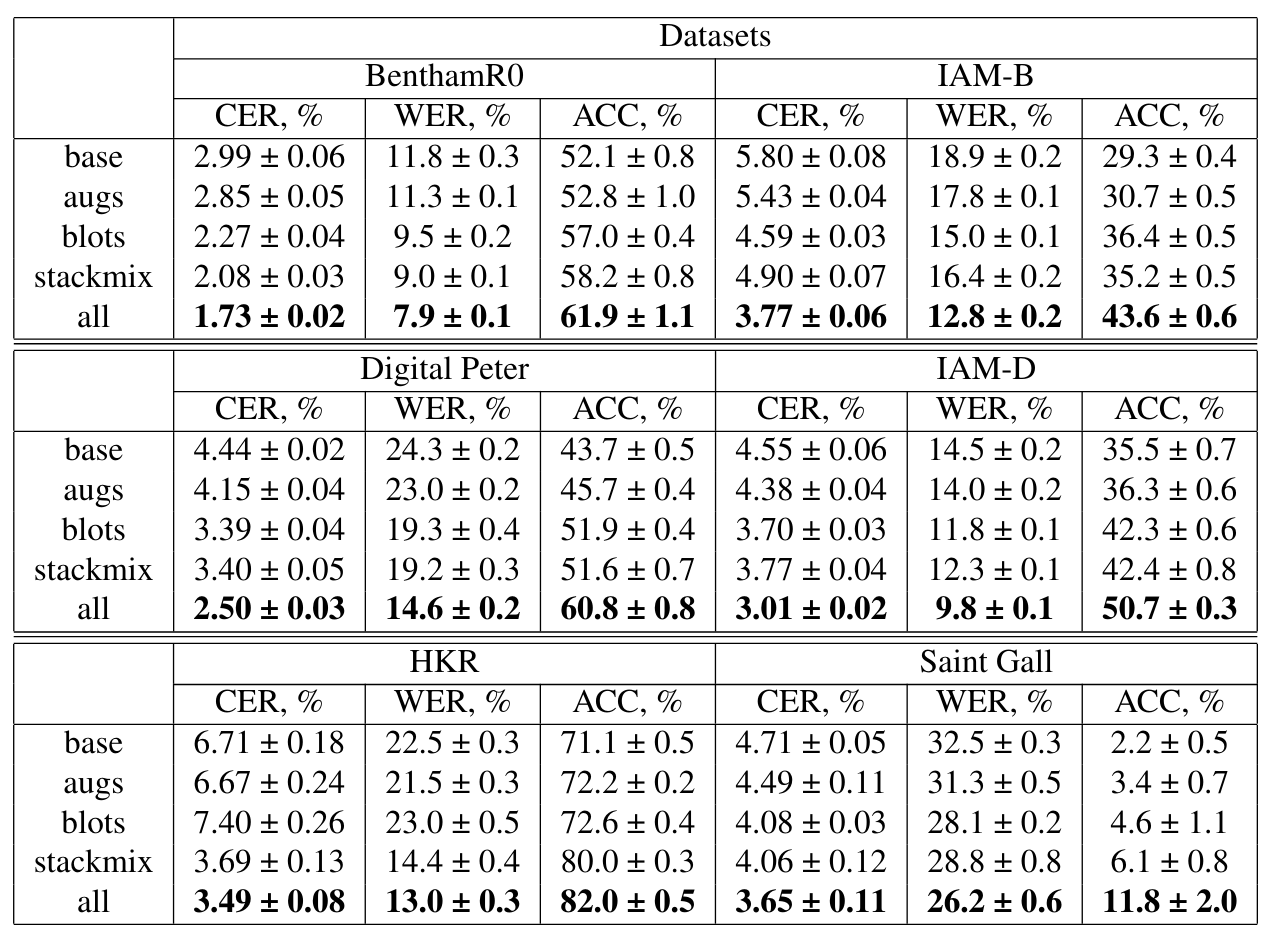
\includegraphics[scale=0.2]{./images/stackmix_results.png}
    \caption{\protect\hypertarget{image9}{Схема постобработки для получения границ символов в StackMix. А также результаты работы. \\ Взято из \protect\hyperlink{cite.Sho21}{[27]}.}}
\end{figure}

Основная идея заключалась в том, чтобы соединить последний слой RNN (после применения активации softmax для каждого символа из функций изображения) и ширину изображения, чтобы получить границы символов, используя только слабо контролируемое обучение без какой-либо ручной разметки \hyperlink{image9}{[Рис 9.]}. Для обучения нейронной сети можно использовать базовую схему без каких-либо дополнений и ухищрений. Для получения качественной разметки границ символов необходимо использовать выборку с этапа обучения.

Один из недостатков данного метода состоит в сильной зависимости от качества алгоритма, определяющего границы символов. Сгенерированные образцы отличаются именно в местах "склейки". В \hyperlink{cite.Sho21}{[27]} одним из свойств датасетов является четкость границы между символами в среднем (это было замечено эмпирически после их анализа). Однако не все рукописные тексты обладают таким качеством.

\subsection{Mixup}

В данном методе предлагается создавать новый образец ($\tilde{x}, \tilde{y}$) следующим образом:
\begin{equation}
\begin{split}
\tilde{x} = \lambda x_i + (1 - \lambda) x_j \\
\tilde{y} = \lambda y_i + (1 - \lambda) y_j
\end{split}
\end{equation}
где $(x_i, y_i)$ и $(x_j, y_j)$ - это два пары ($x$ - вектор признаков, $y$ - целевой объект), выбранные случайным образом из обучающих данных, а $\lambda \sim Beta(\alpha, \alpha), \alpha \in (0, \infty), \lambda \in [0, 1]$. Гиперпараметр $\alpha$ контролирует силу интерполяции между парами признаков-целевых объектов.

Mixup можно понимать как форму аугментации, которая побуждает модель вести себя линейно между по обучающим примерам. Утверждается, что такое линейное поведение уменьшает количество нежелательных колебаний при прогнозировании вне обучающих примеров. Обощением этой идеи является manifold mixup.

\subsubsection{Manifold mixup}

В \hyperlink{cite.Ver18}{[1]} исследователи обнаружили несколько свойств, касающихся скрытых представлений и границ решений современных нейронных сетей. Во-первых, граница решения часто резкая и близка к данным. Во-вторых подавляющая часть пространства признаков соответствует предсказаниям с высокой степенью достоверности, как внутри, так и вне многообразия данных. Руководствуясь этими интуициями, был придуман Manifold Mixup: простой регуляризатор, который устраняет некоторые из этих недостатков путем обучения нейронных сетей на линейных комбинациях скрытых представлений обучающих примеров.

\begin{figure}
    \centering
    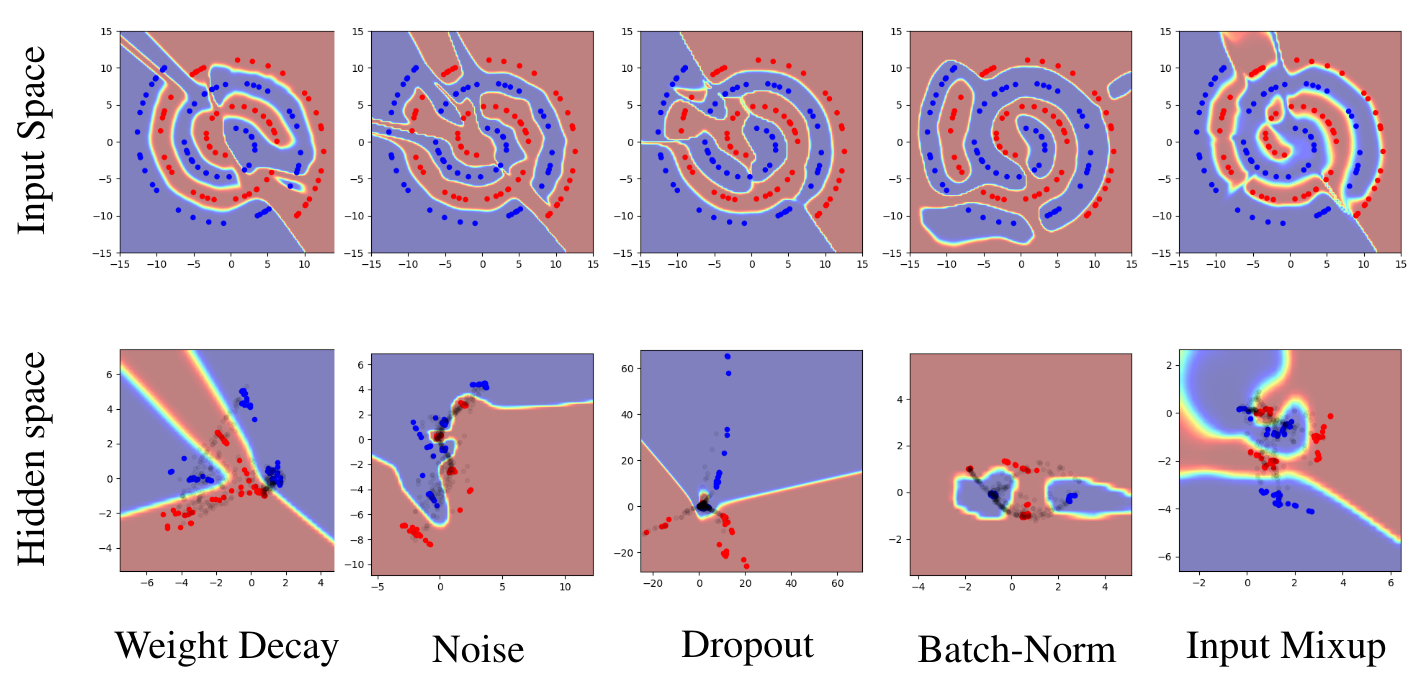
\includegraphics[scale=0.25]{./images/mixup.png}
    \caption{\protect\hypertarget{image10}{Эксперимент с сетью, обученной на 2D наборе спиральных данных с использованием различных регуляризаторов. Эксперимент показывает, что эффект обеспечения широкой области низкой достоверности между областями классов не достигается другими регуляризаторами. Batch Normalization и Dropout на всех слоях, Dropout с вероятностью 0.5, под шумом подразумевается гауссовский шум.
 \\ Взято из \protect\hyperlink{cite.Ver18}{[1]}.}}
\end{figure}

Manifold Mixup улучшает обобщение глубоких нейронных сетей по следующим причинам:
\begin{enumerate}
\item Приводит к более плавным границам принятия решений, которые находятся дальше от обучающих данных, на нескольких уровней пространства признаков. Гладкость и маржа являются общепризнанными факторами генерализации \hyperlink{cite.Pet98}{[28]}.  
\item Использует интерполяцию в более глубоких скрытых слоях, которые собирают информацию более высокого уровня, для обеспечения дополнительного обучающего сигнала.
\item Сглаживает представления классов, значительно сокращая их количество направлений дисперсии (будет описано далее).
\end{enumerate}

\paragraph{Метод}
Рассмотрим обучение глубокой нейронной сети $f(x) = f_k(g_k(x))$, где $g_k$ обозначает часть нейронной сети, отображающую входные данные в скрытое представление на уровне $k$, а $f_k$ обозначает часть, отображающую данное скрытое представление в выход $f(x)$. 

Вначале мы выбираем случайный уровень $k$ из набора допустимых уровней $S$ в нейронной сети. Этот набор может включать в себя самый первый уровень $g_0(x)$. На практике $k$ выбирается равновероятно из некоторых фиксированных уровней.

Далее считается скрытое представление образцов $(x, y)$ и $(x_0, y_0)$ до уровня $k$. После этого есть промежуточные образцы $(g_k(x), y)$ и $(g_k(x_0), y_0)$. На практике $(x, y)$ и $(x_0, y_0)$ берутся из одного батча. Подробности в \hyperref[sec:Chapter3]{Главе 4}.

После слоя $k$ происходит mixup \hyperlink{cite.Hon17}{[25]}:
\begin{equation}
    (\tilde{g_k}, \tilde{y}) = (Mix_{\lambda}(g_k(x), g_k(x_0)), Mix_{\lambda}(y, y_0))
\end{equation}
где $Mix_{\lambda}(a, b) = \lambda \cdot a + (1 - \lambda) \cdot b$. Здесь $(y, y_0)$ - это целевые переменные, а коэффициент $\lambda$ выбирается из распределения $Beta(\alpha, \alpha)$, как и в \hyperlink{cite.Hon17}{[25]}.

Наконец, данное скрытое представление отображается в выход обычным образом и считается функция ошибки.

Формально говоря, Manifold Mixup минимизирует:
\begin{equation}
L(f) = \mathbb{E}_{(x,y) \sim P} \mathbb{E}_{(x_0, y_0) \sim P} \mathbb{E}_{\lambda \sim \text{Beta}(\alpha, \alpha)} \mathbb{E}_{k \sim S} l( f_k\left( \text{Mix}_{\lambda}(g_k(x), g_k(x_0)) \right), \text{Mix}_{\lambda}(y, y_0)).
\end{equation}
где $l$ - функция ошибки, $P$ - распределение входных данных.

\paragraph{Теоретическое обоснование}
Предположим, что $\mathcal{X}$ и $\mathcal{H}$ обозначают пространства входных данных и признаков соответственно. Обозначим целевое множество $\mathcal{Y}$, а $\mathcal{Z} = \mathcal{X} \times \mathcal{Y}$. Пусть $\mathcal{G} \subseteq \mathcal{H}^\mathcal{X}$ обозначает множество функций, реализуемых нейронной сетью, от ввода к данному пространству признаков (до слоя $k$). Аналогично, пусть $\mathcal{F} \subseteq \mathcal{Y}^\mathcal{H}$ будет множеством всех функций, реализуемых нейронной сетью, от представления к ответу. Тогда решение задачи можно описать в следующем виде:

\begin{equation}
J(P) = \inf_{g\in G, f\in F} \mathbb{E}_{(x,y),(x_0, y_0), \lambda} l( f(Mix_\lambda(g(x), g(x_0))), Mix_\lambda(y, y_0))
\end{equation}

Точнее говоря, пусть $P_D$ - эпирическое распределение, $D = \{(x_i, y_i)\}_{i=1}^{n}$. Затем, пусть $f^* \in \mathcal{F}$ и $g^* \in \mathcal{G}$ будут минимизаторами $J(P)$ для $P = P_D$. Также пусть $\mathcal{G} = \mathcal{H}^\mathcal{X}$ и $\mathcal{F} = \mathcal{Y}^\mathcal{H}$, и $\mathcal{H}$ является векторным пространством. Эти условия утверждают, что отображения, реализуемые большими нейронными сетями, плотны во множестве всех непрерывных ограниченных функций. В этом случае мы покажем, что минимизатор $f^*$ является линейной функцией из $\mathcal{H}$ в $\mathcal{Y}$. В таком случае, $J(P)$ может быть переписано следующим образом:

\begin{equation}
J(P_D) = \inf_{h_1,...,h_n \in \mathcal{H}} \frac{1}{n(n-1)} \sum_{i \neq j}^n \inf_{f \in \mathcal{F}} \int_{0
}^{1} l( f(\text{Mix}_{\lambda}(h_i, h_j)), \text{Mix}_{\lambda}(y_i, y_j)) p(\lambda) d\lambda
\end{equation}
где $h_i = g(x_i)$.

\begin{theorem}
Пусть $\mathcal{H}$ - векторное пространство размерности $dim(\mathcal{H})$, и пусть $d \in \mathbb{N}$ обозначает количество классов, содержащихся в датасете $D$. Если $dim (\mathcal{H}) \geq d-1$, то $J(P_D) = 0$ и соответствующий минимизатор $f^*: \mathcal{H} \rightarrow \mathbb{R}^d$ является линейной функцией.
\end{theorem}
\begin{proof}
Сначала заметим, что если $dim(\mathcal{H}) \geq d - 1$, то:
$$ \exists A, H \in \mathbb{R}^{dim(\mathcal{H}) \times d}, b \in \mathbb{R}^{d}: A^T H + b1_{d}^T = I_{d \times d}, $$
где $I_{d \times d}$ и $1_d$ обозначают $d$-мерную единичную матрицу и вектор из единиц соответственно. Фактически,
$b1_{d}^T$ является матрицей ранга один, тогда как ранг единичной матрицы равен $d$. Таким образом, для $A^T H$ достаточно только ранга $d - 1$.

Пусть $f^{*}(h) = A^T h + b$ для всех $h \in \mathcal{H}$. Пусть $g^{*}(x_i) = H_{\zeta_i,:}$ пусть $\zeta_i$-м столбцом матрицы $H$, где
$\zeta_i \in \{1, , d\}$ обозначает индекс класса примера xi. Эти выборы минимизируют (2), так как:
$$ `(f^?(Mix\lambda(g^?(xi), g^?(xj))), Mix\lambda(yi, yj)) = `(A^T Mix\lambda(H{\zeta_i,:}, H{\zeta_j,:}) + b, Mix\lambda(y{i,\zeta_i}, y{j,\zeta_j})) = `(u, u) = 0. $$
Результат следует из $A^T H{\zeta_i,:} + b = y{i,\zeta_i}$ для всех i.
\end{proof}

\paragprah Адаптация к Connectionist temporal classification


\newpage